\documentclass[a4paper]{article}
\usepackage[T1]{fontenc}
\usepackage[utf8x]{inputenc}
\usepackage[margin=1.1in]{geometry}
\usepackage[francais]{babel}
\usepackage{graphicx}
\usepackage{parskip}
\usepackage{float}
\usepackage[procnames]{listings}
\usepackage{color}
\usepackage{hyperref}

\definecolor{darkblue}{rgb}{0.0,0.0,0.7}
\definecolor{darkgreen}{rgb}{0.0,0.5,0.0}

\lstset{
	basicstyle=\ttfamily\small\color{darkblue},
	stringstyle=\color{darkgreen},
	breaklines=true,
	breakatwhitespace=false
}

\usepackage{setspace} % increase interline spacing slightly
\setstretch{1.1}

\title{
	Web Mining \\
	Lab 01 - Crawling, indexation et recherche de pages Web}
\author{
	Damien Rochat, Dorian Magnin \\
	Master of Science in Engineering \\
	HES-Source}
\date{\today}

\begin{document}
	\maketitle
	
	\section{Introduction}
	Le but de ce laboratoire est de mettre en place un système d'indexation et de recherche de contenus provenant de pages Web.
	Nous avons utilisé le logiciel Apache Solr pour l'indexation et développé deux petites applications Java permettant respectivement de crawler
	et indexer des pages Web et d'exécuter des recherches.

	Nous avons choisi de travailler avec le site stackoverflow.com, bien connu des développeurs,
	permettant de répondre à toutes sortes de questions sur le thème de la programmation informatique.
	Le but était de récupérer les questions posées sur le site et de proposer une recherche simple par mot clé,
	celle-ci devant retourner les questions les plus pertinents avec le lien vers la page Web afin d'obtenir d'éventuelles réponses.
	
	\section{Crawler}
	Le crawler (développé avec la librairie Java Crawler4j) va utiliser comme racine, la page d'accueil du site (\url{https://stackoverflow.com/})
	et visiter tous les liens en restant sur le domaine, sans limite de profondeur.
	Ensuite, mêmes si elles sont toutes visitées afin d'obtenir le maximum de contenu,
	seules les pages « question » (au format \url{https://stackoverflow.com/questions/[chiffre]/}) sont indexées.
	En effet, il s'agit des seules pages qui sont intéressantes pour notre application.
	De plus, le crawler mémorise les pages visitées en ne tenant pas compte des paramètres d'URL afin de ne pas indexer plusieurs fois la même page.

	Nous nous sommes très vite heurtés au problème de bannissement du site qui est visiblement très restrictif.
	Après plusieurs tests, nous avons fini par utiliser un taux de 1 requête par secondes (\emph{politeness} de 1000 ms).
	Ceci rend l'indexation lente, mais nous ne subissons plus de blocage.
	Après environ 1 heure, Solr avait indexé plus de 2'600 questions.

	\begin{figure}[H]
		\centering
		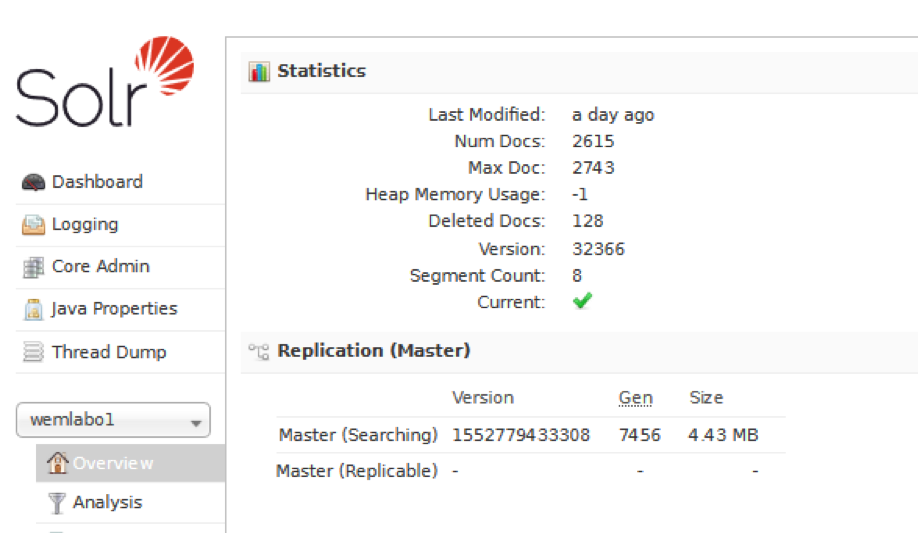
\includegraphics[width=\columnwidth]{images/01-solr-stats.png}
		\caption{Statistiques du cœur Solr après crawling}
	\end{figure}

	Nous n'avons pas rencontré de problème de concurrence. Étant donné le \emph{politeness} assez haut,
	l'attente entre deux mise à jour de l'index est particulièrement élevée.
	
	\section{Indexation spécialisée}
	A l'aide de la librairie jsoup, nous avons récupéré plusieurs informations textuelles dans le code HTML de la page,
	à savoir le titre de la question, son contenu, les tags que l'utilisateur lui a attribué.
	Mais nous avons également récupéré la date de publication de la question, si celle-ci a déjà été résolue ou non,
	ainsi que le nombre de votes positifs qu'elle a reçus de la part de la communauté. Ces quelques champs ne sont pas utiles pour la recherche,
	mais peuvent l'être pour les utilisateurs effectuant une recherche avec notre application.
	
	En résumé, voici la configuration qui a été définie pour les différents champs du cœur Solr :

	\lstset{language=XML}
	\begin{lstlisting}
<field name="id" type="string" indexed="true" stored="true" required="true" multiValued="false" />
<field name="url" type="string" indexed="false" />
<field name="title" type="text_general" multiValued="false" />
<field name="content" type="text_general" multiValued="false" />
<field name="tags" type="text_general" multiValued="true" />
<field name="upvotes" type="pint" indexed="false" />
<field name="answered" type="boolean" indexed="false" />
<field name="date" type="pdate" indexed="false" />
	\end{lstlisting}

	Les champs « url », « upvotes », « answered » et « date » ne sont pas indexés,
	mais simplement stockés afin de pouvoir être affichés dans les résutats de la recherche.
	Ils sont stockés selon leur format correspondant. \\
	Les champs « title » et « content » sont indexés (« text\_general » signifie que les textes seront mis en minuscule, tokenizés et que les stop words seront supprimés). \\
	Finalement, les questions peuvent être liées à plusieurs tags. Le champ « tags » est donc un texte, mais à valeurs multiples.
	L'id du document est défini en hashant l'url de la page, avec la méthode « hashCode() ».
	
	Ci-dessous, un extrait d'une recherche effectuée depuis l'interface Solr.

	\begin{figure}[H]
		\centering
		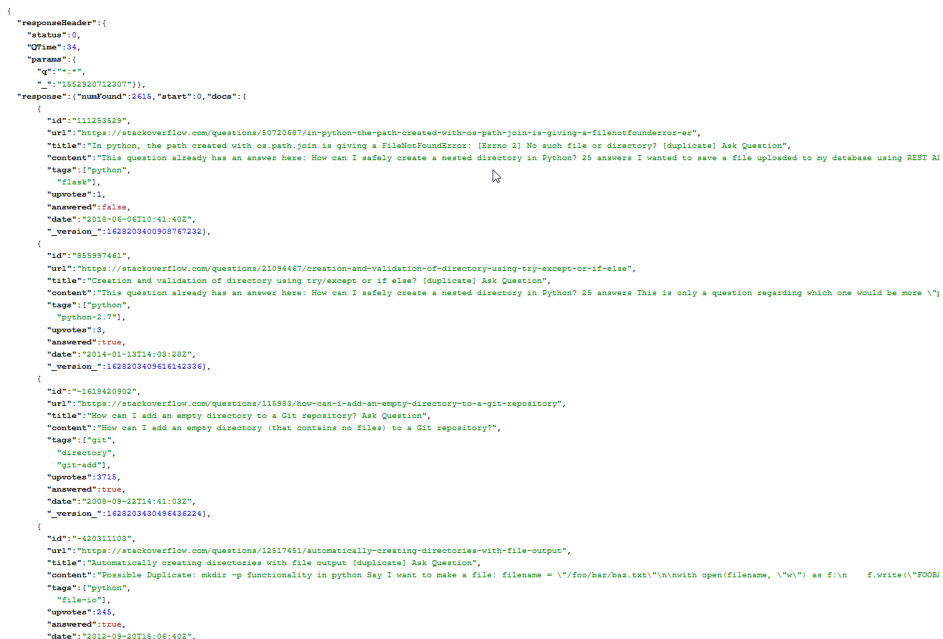
\includegraphics[width=\columnwidth]{images/02-solr-content.png}
		\caption{Recherche de tous les documents dans Solr}
	\end{figure}

	\section{Recherche}
	Concernant la recherche, nous avons utilisé (comme pour l'indexation),
	la librairie solrj. A l'aide de la documentation de Lucene,
	nous avons pu donner plus de poids au titre, puis au tags et enfin au contenu de la question.
	Le code se trouve dans la classe Search. Celle-ci contient une petite application permettant d'entrer un mot clé et d'afficher les résultats de la recherche,
	ordré par pertinence, le tout en mode console.
	
	La première requête Solr que nous avons mise en place était la suivante :

	\begin{verbatim} 
		(title:[SEARCH])^3 (tags:[SEARCH])^2 (content:[SEARCH])^1
	\end{verbatim}

	Les puissances sont utilisées afin de donner plus ou moins d'importance aux différents champs. \\
	En recherchant « stack trace in Java », chaque mot est recherché par Lucene. Voici le résultat correspondant :

	\begin{figure}[H]
		\centering
		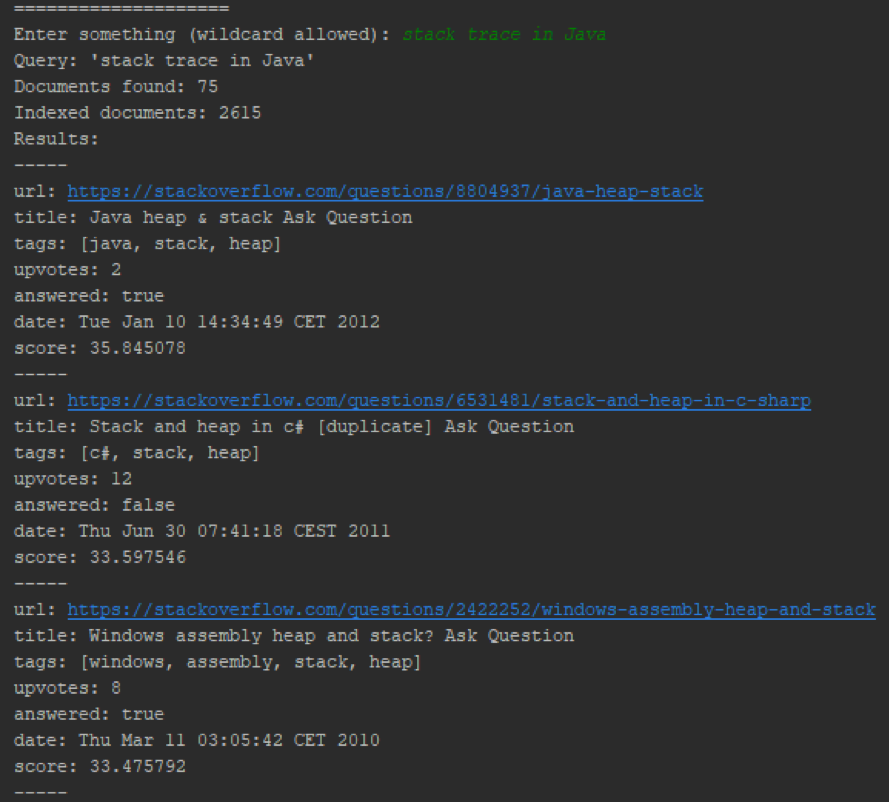
\includegraphics[width=\columnwidth]{images/03-search-01.png}
		\caption{Résultat de la recherche sans optimisation}
	\end{figure}

	Nous avons ensuite amélioré la requête afin de rechercher le terme exacte (la phrase complète) dans le titre,
	en modifier la requête comme ceci :

	\begin{verbatim} 
		(title:"[SEARCH]")^3 (tags:[SEARCH])^2 (%s:[SEARCH])^1
	\end{verbatim}

	Voici le résultat correspondant :

	\begin{figure}[H]
		\centering
		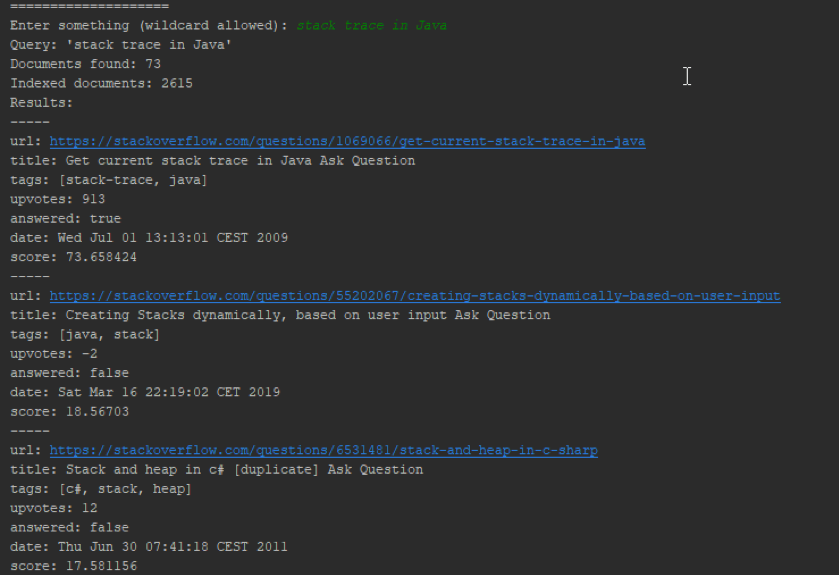
\includegraphics[width=\columnwidth]{images/04-search-02.png}
		\caption{Résultat de la recherche avec terme exacte dans le titre}
	\end{figure}

	Cependant, les autres documents se retrouvent fortement défavorisés,
	leur titre n'étant plus pris en considération s'ils ne possèdent pas le terme exact.

	En mixant les deux requêtes, nous sommes arrivés à obtenir des scores adéquats pour chaque question.
	
	\begin{verbatim} 
		(title:"[SEARCH]")^4 (title:[SEARCH])^3 (tags:[SEARCH])^2 (%s:[SEARCH])^1
	\end{verbatim}

	\begin{figure}[H]
		\centering
		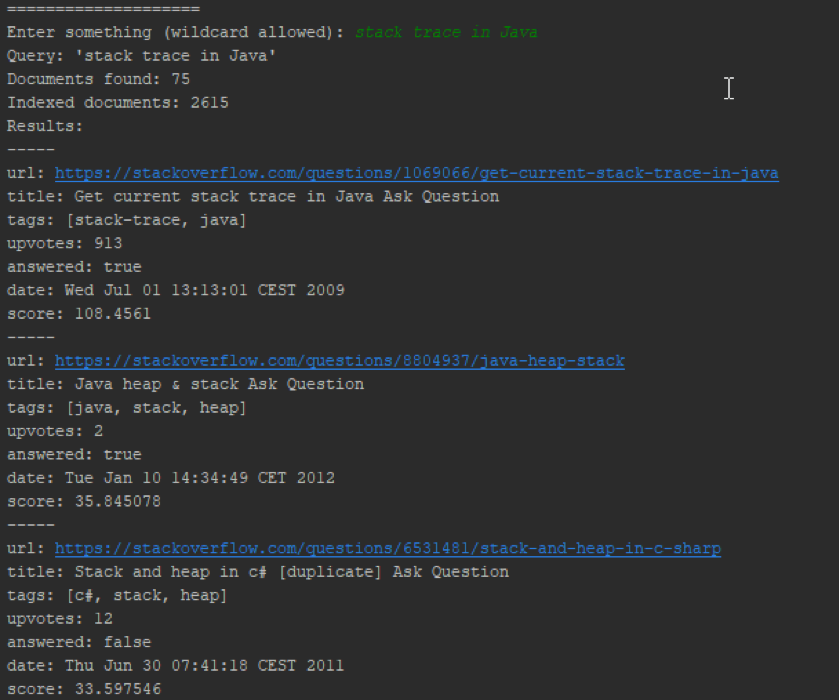
\includegraphics[width=\columnwidth]{images/05-search-03.png}
		\caption{Résultat de la recherche avec optimisation finale}
	\end{figure}

	La recherche pourrait encore être améliorée.
	Sur l'image ci-dessus, on voit bien que les documents retournés de concernent pas Java
	ou ne concerne pas la stack trace (même si leur score est clairement inférieur à celui du premier document).
	Ceci peut provenir du fait que finalement peu de documents ont été indexés.

	\section{Questions théoriques}

	\subsection{Question 1}
	{\bfseries
	Veuillez expliquer quelle stratégie il faut adopter pour indexer des pages dans plusieurs langues
	(chaque page est composée d'une seule langue, mais le corpus comporte des pages dans plusieurs langues).
	A quoi faut-il faire particulièrement attention ? Veuillez expliquer la démarche que vous proposez. 
	}

	La langue peut être indiquée dans l'URL ou dans le header de la requête HTTP (« Content-Language »)
	ou dans le HTML (attribut « lang » de la balise « head »).
	Dans des cas plus compliqués, il pourrait être possible d'analyser les textes de la page Web
	afin d'en déduire la langue à l'aide d'une reconnaissance de certains mots-clés spécifiques à chaque langue.
	Selon le fonctionnement du site Web, il peut être nécessaire d'adapter la requête HTTP envoyée par le crawler en ajouter un header « Accept-Language »,
	voir même un paramètre POST afin de spécifier au serveur la langue que l'on souhaite.

	Une fois celle-ci définie, le crawler va pouvoir filtrer les contenus en fonction des langues à indexer.
	Deux solutions existent concernant Solr :

	\begin{itemize}
		\item Utiliser plusieurs cœurs, un par langue. Cette approche est simple,
		mais va utiliser plus d'espace de stockage.
		\item Utiliser un seul cœur et dupliquer les champs « traduisibles » (e.g. « title\_de », « title\_fr »).
		Avec cette méthode, les données communes aux différents languages ne seront pas dupliquées
		et il n'y a qu'un seul cœur à administrer, indépendemment du nombre de langues.
	\end{itemize}

	\subsection{Question 2}
	{\bfseries
	Solr permet par défaut de faire de la recherche floue (fuzzy search).
	Veuillez expliquer de quoi il s'agit et comment Solr l'a implémenté.
	Certains prénoms peuvent avoir beaucoup de variation orthographiques
	(par exemple Caitlin : Caitilin, Caitlen, Caitlinn, Caitlyn, Caitlyne, Caitlynn,
	Cateline, Catelinn, Catelyn, Catelynn, Catlain, Catlin, Catline, Catlyn, Catlynn,
	Kaitlin, Kaitlinn, Kaitlyn, Kaitlynn, Katelin, Katelyn, Katelynn, etc).
	Est-il possible d'utiliser, tout en gardant une bonne performance,
	la recherche floue mise à disposition par Solr pour faire une recherche prenant en compte de telles variations ?
	Sinon quelle(s) alternative(s) voyez-vous, veuillez justifier votre réponse. 
	}

	Les requêtes « floues » (FuzzyQuery) permettent de spécifier une distance maximale entre le terme recherché
	et les termes qui pourront être retournés, selon les algorithmes Damerau-Levenshtein Distance ou Edit Distance.
	Les résultats ne seront donc pas exactement similaires, mais proches. Ensuite, le score des résultats prendront en compte leur distance respective. \\
	Par exemple, « Caitlin~1 » matchera « Caitilin », « Caitlen », « Caitlinn » ou encore « Caitlyn » qui ont une différence d'un caractère chacun.

	Pour des raisons de performance et de précision du résultat,
	il n'est cependant pas conseillé d'utiliser une distance trop importante (2 au maximum).
	Le stemming (réduire les termes similaires à un terme commun) peut être utilisé comme alternative dans une majorité des cas.

	\section{Conclusion}
	Ce travail nous a permis de mettre assez facilement en place un moteur de recherche pour un site tiers.
	Cependant, nous nous sommes également rendu compte que crawler un site tel que stackoverflow qui contient énormément de contenu
	et très long, de plus de nouveaux contenus apparaissent et sont modifiés de manière continue ce qui rend l'indexation difficile.

	Finalement, même si une simple recherche est aisée à mettre en place,
	arriver à obtenir les résultats les plus relevants possible nécessite d'implémenter une multitude de techniques
	(e.g. recherche floue, stemming), de trouver et de pondérer les bons éléments.

\end{document}
